\section{Datathons}

% Description of datahton
A datathon is an event similar to a hackathon where people come together over a certain time period, commonly 24 hours to work on problems with a specific dataset. There are a number of steps involved in a datathon including preparing, planning, recruiting participants, arranging an appropriate venue, preparing the data for exploration, logistics, and hosting the event. We describe the benefits of datathons and outline our experience at running four datathons.

\subsection{Benefits}

%------------------------------------------------------------
%         DFG
%------------------------------------------------------------
\subsection{Data For Good Case Study}


Data for Good (DFG)\footnote{http://www.meetup.com/Data-for-Good-Calgary/} is a community organization inspired by DataKind.org and is working for positive social action through ``data in the service of humanity". Data for Good in Calgary brings together data scientists with social organizations through a  collaborative approach that leads to shared insights, greater understanding, and positive action of data. Data for Good leads a community of data scientists from the community and university to inspire a new way of using the skills and tools of corporations \& governments, to meet the needs of the NFP/NGO and social innovation sector.

DDG organizes regular meetups for it's members and hosts weekend datathon events. A DataThon is a weekend event that matches up selected social organizations (that have well-defined data problems) with a team of volunteer data scientists to tackle their data-related challenges over a 24-48 hours period. The participants are fed throughout the weekend event \& the results are presented to the social organizations at the end of the event. Some may refer to these types of events as "Hack-a-Thons", etc. These events are completely free for the participants and serve to energize, educate, and provide direct benefit to the NFP/NGO organizations, as well as to enlighten social sector groups about the power of being data-driven.


Suatainable Alberta Association\footnote{http://www.meetup.com/Data-for-Good-Calgary/events/175671942/}

Distree Centre\footnote{http://www.meetup.com/Data-for-Good-Calgary/events/221869098/}


%------------------------------------------------------------
%         CODE
%------------------------------------------------------------
\subsection{Canadian Open Data Experience (CODE) Case Study}

The Canadian Open Data Experience (CODE)\footnote{https://www.canadianopendataexperience.ca/} is an intense 48-hour coding sprint where innovators from coast to coast compete to build the best app utilizing federal government data from Canada's Open Government portal. We organized two hubs as part of the CODE competition in 2014 and 2015. 

In 2014 four teams participated with four members per team.  One team made the grand final of the top 15 teams and presented their app in front of judges in Toronto.

\begin{figure*}[!htb] % this puts images exactly where you want them
\begin{center}
\subfigure[CODE 2014 - Brainstorming Session.]{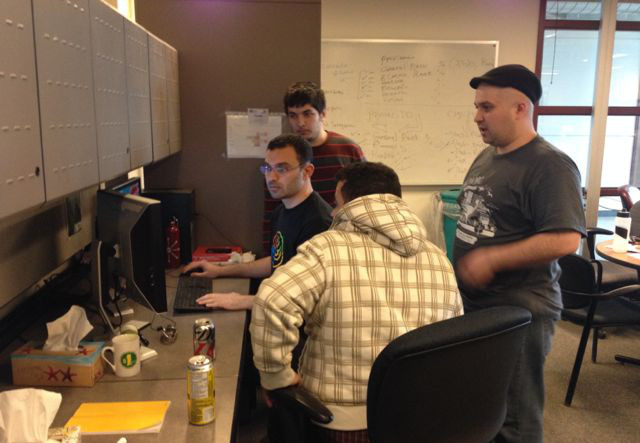
\includegraphics[keepaspectratio,width=8cm]{images/code-2014-brainstorm.jpg}\label{fig:brainstorm}}
\subfigure[Data For Good 2014 - Introductory Session.]{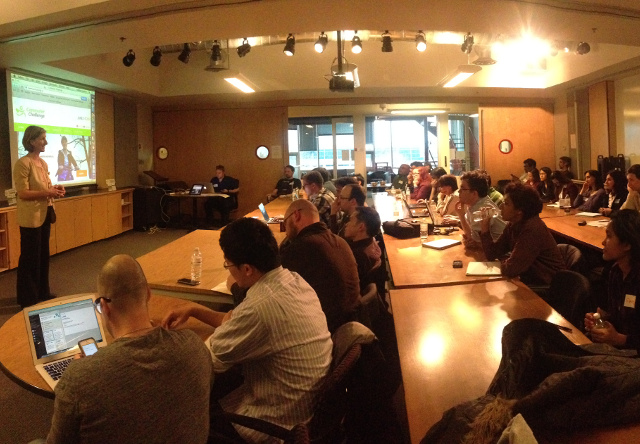
\includegraphics[keepaspectratio,width=8cm]{images/dfg-2014-introductory.jpg}\label{fig:sdv}}
\caption{Datathons Case Study - illustrating different aspects of the datathons.}
\label{fig:datathons}
\end{center}
\end{figure*}